% 
% Annual Cognitive Science Conference
% Sample LaTeX Paper -- Proceedings Format
% 

% Original : Ashwin Ram (ashwin@cc.gatech.edu)       04/01/1994
% Modified : Johanna Moore (jmoore@cs.pitt.edu)      03/17/1995
% Modified : David Noelle (noelle@ucsd.edu)          03/15/1996
% Modified : Pat Langley (langley@cs.stanford.edu)   01/26/1997
% Latex2e corrections by Ramin Charles Nakisa        01/28/1997 
% Modified : Tina Eliassi-Rad (eliassi@cs.wisc.edu)  01/31/1998
% Modified : Trisha Yannuzzi (trisha@ircs.upenn.edu) 12/28/1999 (in process)
% Modified : Mary Ellen Foster (M.E.Foster@ed.ac.uk) 12/11/2000
% Modified : Ken Forbus                              01/23/2004
% Modified : Eli M. Silk (esilk@pitt.edu)            05/24/2005
% Modified : Niels Taatgen (taatgen@cmu.edu)         10/24/2006
% Modified : David Noelle (dnoelle@ucmerced.edu)     11/19/2014

%% Change "letterpaper" in the following line to "a4paper" if you must.

\documentclass[10pt,letterpaper]{article}

\usepackage{cogsci}
\usepackage{pslatex}
\usepackage{apacite}

\usepackage{tikz}
\usetikzlibrary{arrows,shapes,snakes,automata,backgrounds,petri}

\title{Curiosity-Driven Development of Tool Use Precursors}
 
\author{{\large \bf S\'ebastien Forestier (sebastien.forestier@inria.fr)} \\
	INRIA Bordeaux Sud-Ouest\\
	Bordeaux, France
  \AND {\large \bf Pierre-Yves Oudeyer (pierre-yves.oudeyer@inria.fr} \\
	INRIA Bordeaux Sud-Ouest\\
	Bordeaux, France}

\usepackage[caption=false,font=footnotesize]{subfig}


\begin{document}

\maketitle


\begin{abstract}
This is the abstract.

\textbf{Keywords:} 
curiosity-driven learning; tool use; goal babbling; overlapping waves; 
\end{abstract}


\section{Introduction}

	Development of tool use \cite{guerin2013survey}, precursors of tool use: behavior without objects, behavior with one object, interaction of objects.	
	Grounding of representation and planning based on a large amount of experiences. 	
	Seemless progression between the successives phases as overlapping waves. 	
	Ongoing process of upgrading representations.	
	Developmental trajectories.
	
	
	Curiosity studies in developmental psychology 
	\cite{kidd}
	\cite{gottlieb_information-seeking_2013}
	
	Curiosity-driven modelling work, emergence of developmental trajectories.
	\cite{oudeyer_intrinsic_2007} 
	\cite{oudeyer_what_2007}
	\cite{flow}
	\cite{sch}
	\cite{santucci2013}
	\cite{cangelosi2010integration}
	\cite{oudeyer2014evolution}
	
	
	IAC series of architectures and Explauto framework: previous experiments.
	\cite{moulin-frier_self-organization_2014}
	\cite{moulin-frier_explauto:_2014}
	\cite{baranes2010intrinsically}
	\cite{riac}
	\cite{baranes_active_2013}
	
	Representations in explauto and other models 
	\cite{mugan2009}
	\cite{metzen2013}
	\cite{horde}
	\cite{mugan}
	\cite{vig}
	\cite{sutton1999between}
	
	Other related work
	\cite{ugur2015}
	\cite{schmerlinggoal}

	More details on experiments
	\cite{ijspeert_dynamical_2013}
	
	\cite{}
	
%

\section{Methods}

	\subsection{Environment}
	
		\paragraph{}
		We simulate a 2D robotic arm using tools to move an object into different boxes in the environment. 		
		In each trial, we execute a motor command given by the agent, we evaluate its consequences on the sensory dimensions and we give him
		this sensory feedback. Finally the environment is resetted to its intial state.
		
		The next sections precisely describe the different items of the environment and their interactions.	
		See Fig. \ref{env} for an exemple of the state of the environment. 
		
		\begin{figure}[h]
			\centering
			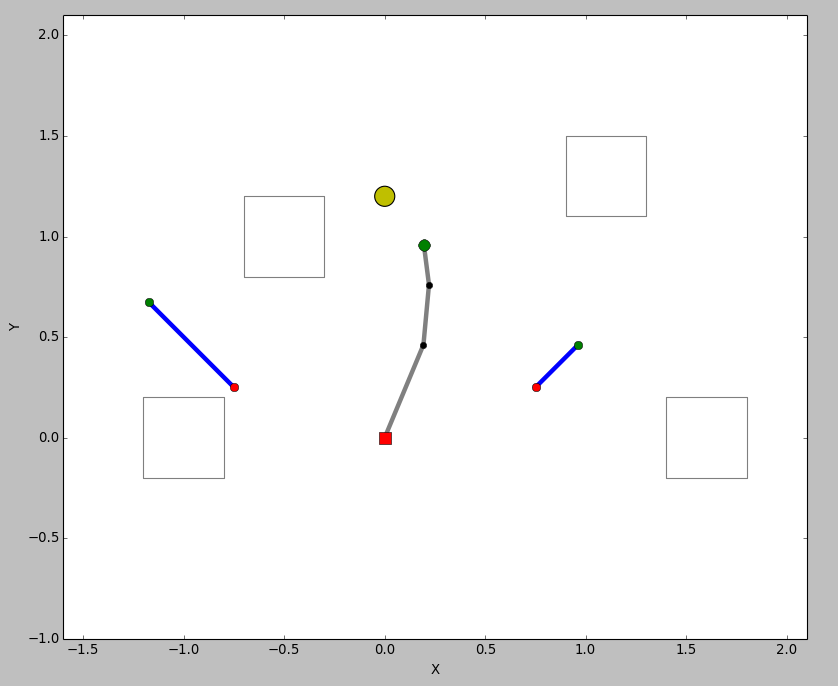
\includegraphics[width=8cm]{./include/tools.png}
			\caption{Play Environment}
			\label{env}
		\end{figure}
			

		\subsubsection{Robotic arm}
		
			The 2D robotic arm has 3 joints plus a gripper located at the end-effector.
			Each joint can rotate from $-\pi~rad$ to $\pi~rad$ around its initial position, mapped to a standard interval of $[-1,1]$.
			The length of the 3 parts of the arm are $0.5$, $0.3$ and $0.2$ so the total length of the arm is $1$ unit.
			The initial position of the arm is vertical with each joint at $0~rad$ and its base is fixed at position $[0, 0]$.
			The gripper $g$ has 2 possible positions: \textit{open} ($g \geq 0$) and \textit{closed} ($g < 0$) and its initial position is \textit{open} (with $g = 0$).
			The robotic arm thus has 4 degrees of freedom represented by a vector in $[-1,1]^4$.
			A trajectory of the arm will be represented as a sequence of such vectors.
		
		%
		
			
		\subsubsection{Objects and tools}
			
			A yellow sphere can be moved into one of the 4 fixed squared boxes. 
			The initial position of the sphere is $(0, 1.2)$ and is thus unreachable directly with the gripper.
			One of two sticks can be grasped in order to reach the object.
			A small stick of length $0.3$ is located on the right of the arm, with initial position $(0.75, 0.25)$ and initial angle $\frac{\pi}{4}$ from the horizontal line.
			A long stick of length $0.6$ is located on the left of the arm, with initial position $(-0.75, 0.25)$ and initial angle $\frac{3\pi}{4}$ from the horizontal line as in Fig. \ref{env}.			
			If the gripper closes near the end of one of the sticks (closer than $0.1$), it is considered grasped and will follow the gripper's position and the angle of the arm's last part until the gripper opens.			
			Similarly, if the other end of a stick reaches the sphere (within $0.1$), the object will follow the end of the stick.
			Ten boxes are static at positions $(-1, 0)$, $(-0.5, 1)$, $(1.1, 1.3)$ and $(1.6, 0)$ and have size $0.2$, 
			so that the two boxes on the left can be reached by the two sticks, and the two boxes on the right can only be reached by the long stick.
			At the end of the trial, the object is considered to be in one of the box if its center is in the box.\\
		
		%
		
		\subsubsection{Motor control}
		
			We use Dynamical Movement Primitive \cite{ijspeert_dynamical_2013} to control the arm's movement as this framework permits the production of a diversity of arm's trajectories with few parameters.
			Each of the $4$ arm's degrees-of-freedom (DOF) is controlled by a DMP with a starting and a goal position equal to the rest position of the joint.
			Each DMP is parameterized by one weight on each of $3$ basis functions whose centers are distributed homogeneously throughout the movement duration.
			The weights are bounded in the interval $[-200,200]$ (mapped to the standard interval $[-1,1]$) which allow each joint to fairly cover the interval $[-1,1]$ during the movement.
			Each DMP outputs a series of $50$ positions that represents a sampling of the trajectory of one joint during the movement.		
			The arm's movement is thus parameterized by $12$ weights which are represented by the motor space $M=[-1,1]^{12}$
		
		%
		
		\subsubsection{Sensory feedback}
		
			At the end of the movement, the robot gets sensory feedback from the different items of the environment.
			It gets the trajectory of its hand and gripper, the trajectory of the end of the sticks, 
			the end position of the object, and whether the object is in each box.		
			The trajectory of the hand and of the end point of the sticks are represented by sequences of x and y positions at different time points: 
			steps $12$, $25$, $37$ during the movement of $50$ steps ($6$D for the hand and for each stick).
			Similarly, the trajectory of the gripper is a sequence of $1$ or $-1$ depending whether the gripper is open or closed ($3$D).
			For each box, the robot receives a $1$ if the object is in the box at the end of the movement, and $0$ otherwise ($4$D).			 
			The sensory information thus contains $9$ values for the trajectory of the hand and gripper, $6$ for the trajectory of the end of each stick, $2$ for the end position of the object and $4$ for the boxes.
			The sensory space has a total of $27$ dimensions.
			
		%
		
	%
	
	\subsection{Learning architectures}

		\subsubsection{Explauto framework}
			
			\cite{moulin-frier_explauto:_2014}
			
				
		%
		
		\subsubsection{Goal Babbling}
			
				
		%
		
		\subsubsection{SAGG-RIAC}
			
			\cite{baranes_active_2013}
			
				
		%
		
		\subsubsection{Flat architecture}
			
				
		%
		
		\subsubsection{Hierarchical architecture}
			
			We present here an architecture that represents sensorimotor information with a hierarchical structure.
			
			\begin{figure}[t]
				\center
				
% H2
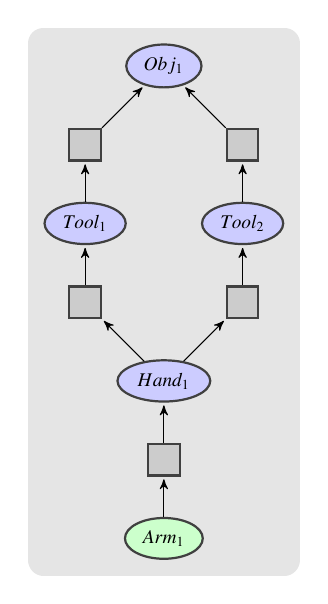
\begin{tikzpicture}[node distance=1.cm,>=stealth',bend angle=45,auto]

	\tikzstyle{dom}   = [ellipse, thick, draw=black!75, fill=blue!20,  minimum height=5mm, minimum width=5mm]
	\tikzstyle{prim dom}   = [dom,  minimum height=5mm, minimum width=5mm,  fill=green!20]
	\tikzstyle{mod} = [rectangle, thick, draw=black!75, fill=black!20, minimum size=4mm]

	\begin{scope}
		\scriptsize
		\node [prim dom] (pd1) {$Arm_1$};
		
		\node [mod] (m1) [above of=pd1] {}
		edge [pre]                  (pd1);

		\node [dom] (d1) [above of=m1] {$Hand_1$}
		edge [pre]                (m1);
		
		\node [mod] (m2) [above of=d1, xshift=-1cm] {}
		edge [pre]                  (d1);
		
		\node [mod] (m3) [right of=m2, xshift=1cm] {}
		edge [pre]                  (d1);
		
		\node [dom] (d2) [above of=m2] {$Tool_1$}
		edge [pre]                (m2);
		
		\node [dom] (d3) [above of=m3] {$Tool_2$}
		edge [pre]                (m3);
		
		\node [mod] (m4) [above of=d2] {}
		edge [pre]                  (d2);
		
		\node [mod] (m5) [above of=d3] {}
		edge [pre]                  (d3);
		
		\node [dom] (d4) [above of=m4, xshift=1cm] {$Obj_1$}
		edge [pre]                (m4)
		edge [pre]                (m5);
		
		
	\end{scope}
	\begin{pgfonlayer}{background}
		\filldraw [line width=4mm,join=round,black!10]
		(d4.north  -| d3.east)  rectangle (pd1.south  -| d2.west);
	\end{pgfonlayer}
\end{tikzpicture}

				\caption{Hierarchy of sensorimotor models}
				\label{H}					
			\end{figure}

				
		%
		

	%
	
	\subsection{Experiments}
		
		NN, 100 iterations of Motor babbling and then 300000 iterations of the condition
		
		Only the motor module (mod1) adds exploration noise ($\sigma=0.02$) even in hierarchical architecture.
		
		\subsubsection{Conditions}
			
			\begin{itemize}
			
				\item H0-MB: Random Motor Babbling
				\item H0-GB: Random Goal Babbling with a flat architecture learning $$M \rightarrow S_{Hand} \times S_{Stick_1} \times S_{Stick_2} \times S_{Object} \times S_{Boxes}$$
				\item H0-TR: The same architecture but with active goal babbling (my version of SAGG-RIAC)
				\item H1: Hierarchical architecture with Random Goal Babbling in each module, and choice of module that babbles based on interest ($\epsilon$-prop: probabilities proportional to interest but with $\epsilon=10\%$ of random choice). Choice of tool to use based on the maximum interest of the two modules that learn from the spaces of the tools to the object space, around the goal object point (competence progress on the k=10 NN).
				\item H1-GR: same as H1 but the choice of module to babble is $\epsilon$-greedy with $\epsilon=0.1$
				\item H1-CL: same as H1 but the choice of the tool to use is based on the maximum competence around the goal object point (competence of the NN)
			
			\end{itemize}
				
		%
		
		\subsubsection{Measures}
			
			Exploration of the different sensory spaces (number of reached cells in a discretization of the space divided by number of cells).
				
		%
		
	%
	
%


\section{Results}


		\begin{figure*}[ht]
			\centering
			\subfloat[Hand]{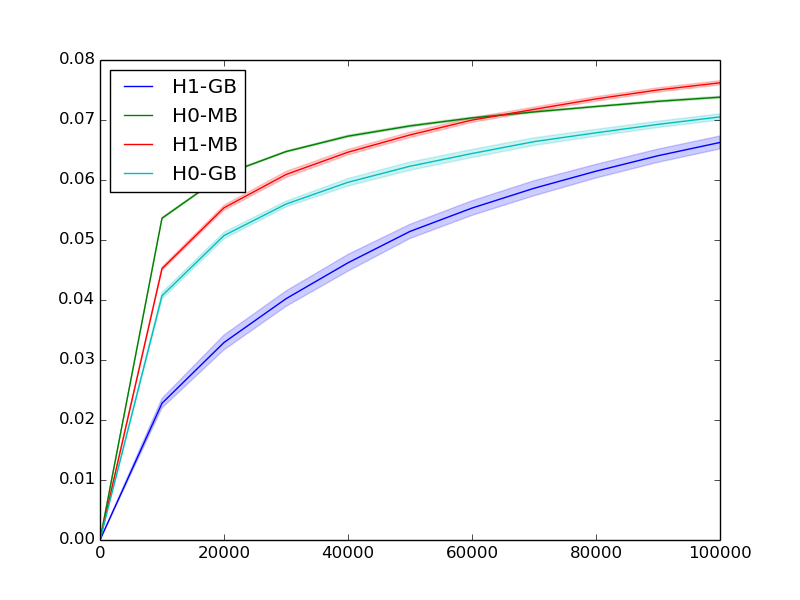
\includegraphics[width=4.5cm]{./include/xp1-explo-hand.png}}
			\subfloat[Tool]{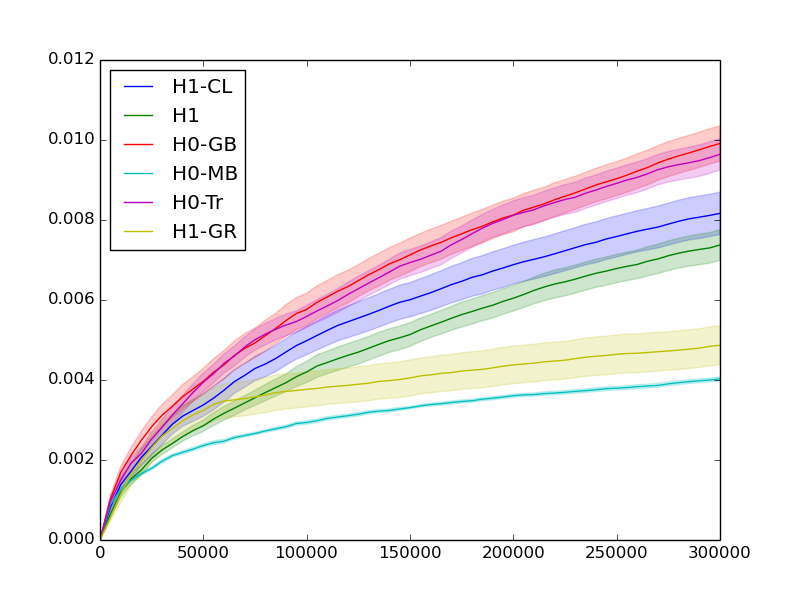
\includegraphics[width=4.5cm]{./include/xp1-explo-stick_1.png}}
			\subfloat[Object]{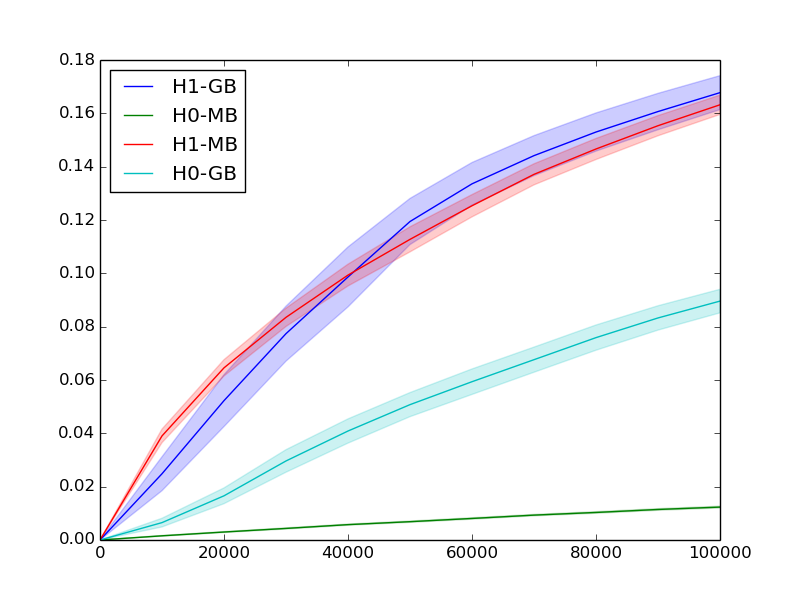
\includegraphics[width=4.5cm]{./include/xp1-explo-obj.png}}
			\subfloat[Box]{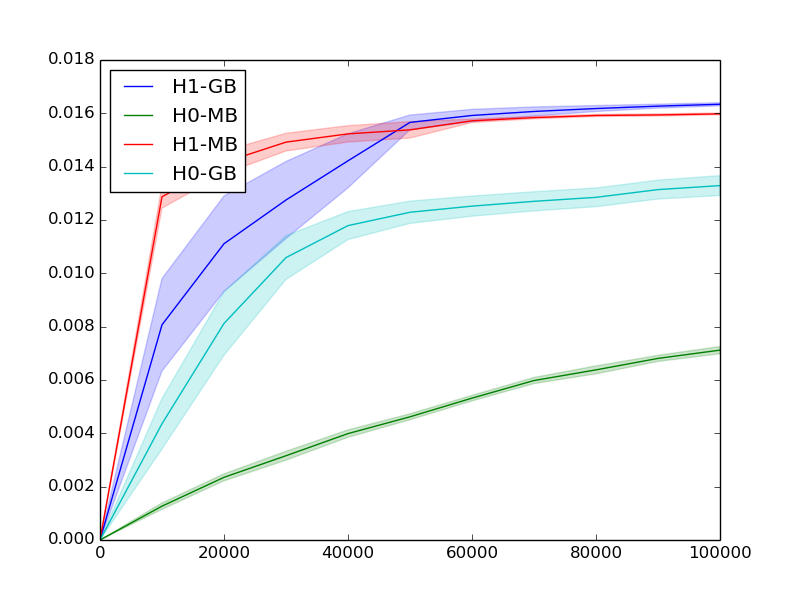
\includegraphics[width=4.5cm]{./include/xp1-explo-box.png}}
			\caption{Exploration of sensory spaces.}
			\label{res_explo}
		\end{figure*}
	
	
		\begin{figure*}[ht]
			\subfloat[]{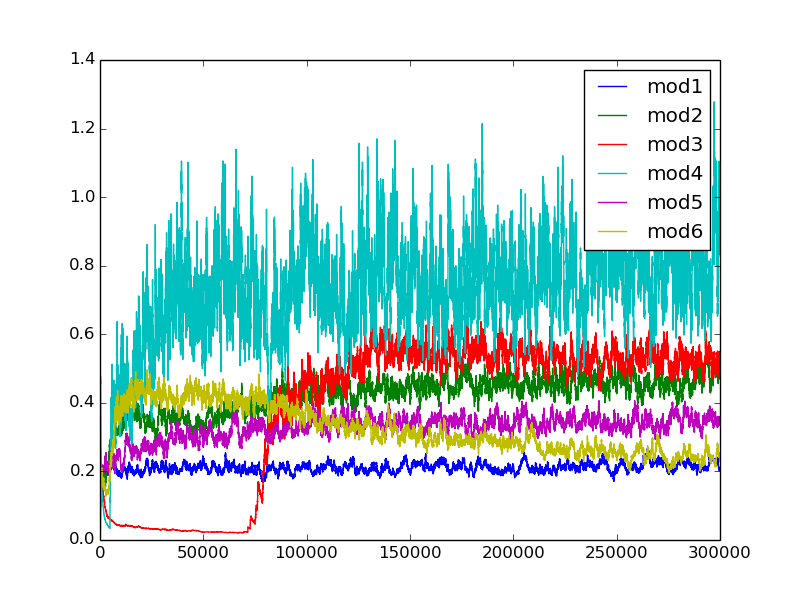
\includegraphics[width=9cm]{./include/H1-log3-interests.png}}
			\subfloat[]{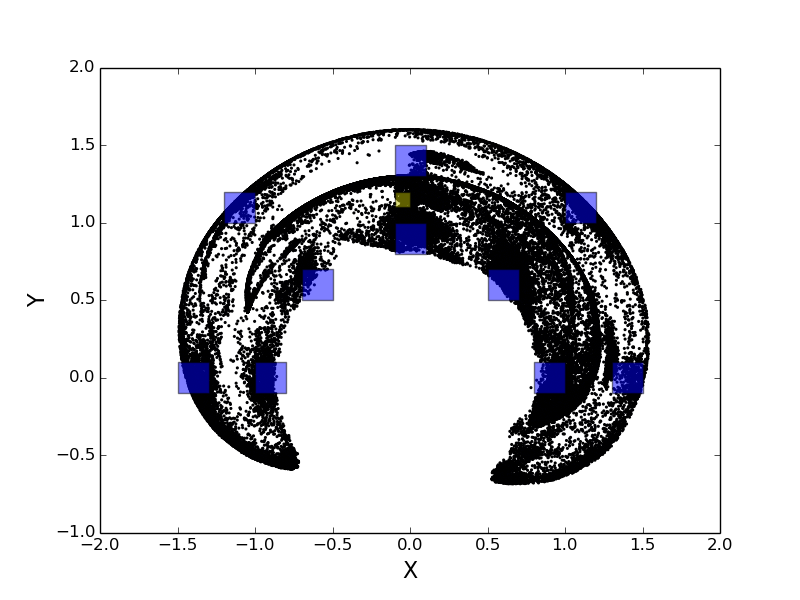
\includegraphics[width=9cm]{./include/H1-log3-obj-explo.png}}
			\caption{Condition H1. (a) Interests of each module. (b) Exploration of the object space: each dot is one point reached with the object at the end of one movement.}
			\label{res_interests}
		\end{figure*}
	
	
		\begin{figure*}[ht]
			\subfloat[H1]{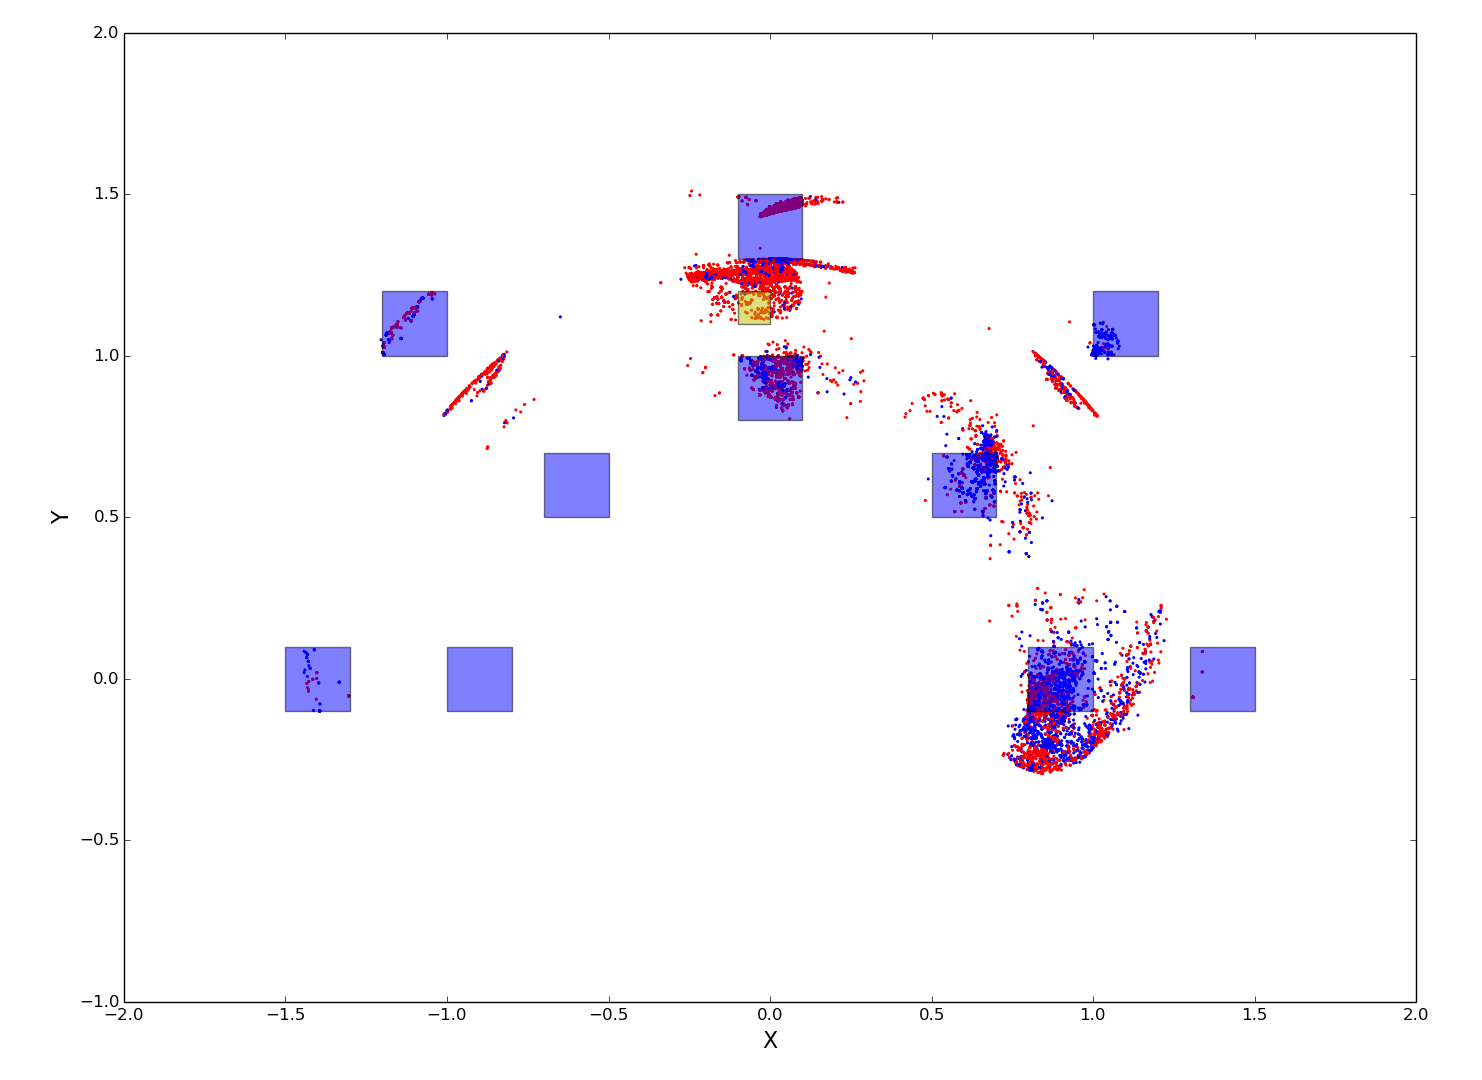
\includegraphics[width=9cm]{./include/choice_mod4_H1.png}}
			\subfloat[H1-CL]{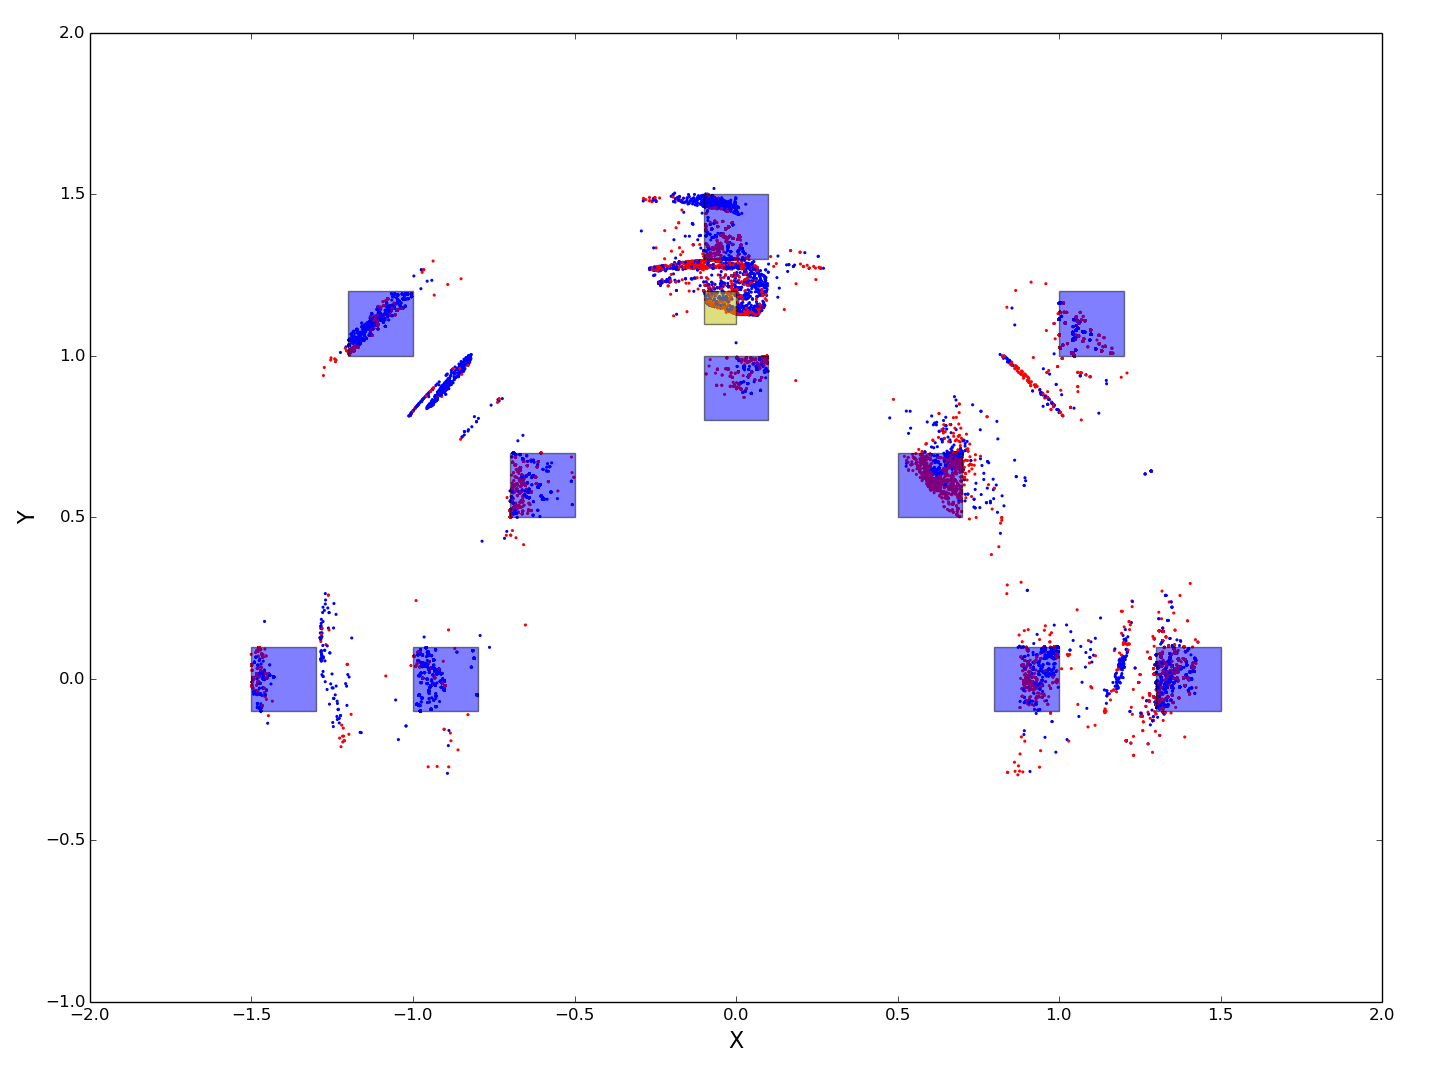
\includegraphics[width=8.8cm]{./include/choice_mod4_H1-CL.png}}
			\caption{Chosen tool depending on object goal position. Blue points: long stick choice. Red points: small stick choice.}
			\label{res_choice}
		\end{figure*}
	
%


\section{Discussion}

	\subsection{H0 vs H1}
	
	
	%

	\subsection{H1 vs H1-GR}
	
	
	%
	
	\subsection{H1 vs H1-CL}
	
	
	%
	
%


\section{Acknowledgments}

%




\bibliographystyle{apacite}

\setlength{\bibleftmargin}{.125in}
\setlength{\bibindent}{-\bibleftmargin}

\bibliography{include/bibliography}


\end{document}
